\documentclass[a4paper, 14pt]{extarticle}

% Поля
%--------------------------------------
\usepackage{geometry}
\geometry{a4paper,tmargin=2cm,bmargin=2cm,lmargin=3cm,rmargin=1cm}
%--------------------------------------


%Russian-specific packages
%--------------------------------------
\usepackage[T2A]{fontenc}
\usepackage[utf8]{inputenc} 
\usepackage[english, main=russian]{babel}
%--------------------------------------

\usepackage{textcomp}

% Красная строка
%--------------------------------------
\usepackage{indentfirst}               
%--------------------------------------             


%Graphics
%--------------------------------------
\usepackage{graphicx}
\graphicspath{ {./images/} }
\usepackage{wrapfig}
%--------------------------------------

% Полуторный интервал
%--------------------------------------
\linespread{1.3}                    
%--------------------------------------

%Выравнивание и переносы
%--------------------------------------
% Избавляемся от переполнений
\sloppy
% Запрещаем разрыв страницы после первой строки абзаца
\clubpenalty=10000
% Запрещаем разрыв страницы после последней строки абзаца
\widowpenalty=10000
%--------------------------------------

%Списки
\usepackage{enumitem}

%Подписи
\usepackage{caption} 

%Гиперссылки
\usepackage{hyperref}

\hypersetup {
	unicode=true
}

%Рисунки
%--------------------------------------
\DeclareCaptionLabelSeparator*{emdash}{~--- }
\captionsetup[figure]{labelsep=emdash,font=onehalfspacing,position=bottom}
%--------------------------------------

\usepackage{tempora}

%Листинги
%--------------------------------------
\usepackage{listings}
\lstset{
  basicstyle=\ttfamily\footnotesize, 
  %basicstyle=\footnotesize\AnkaCoder,        % the size of the fonts that are used for the code
  breakatwhitespace=false,         % sets if automatic breaks shoulbd only happen at whitespace
  breaklines=true,                 % sets automatic line breaking
  captionpos=t,                    % sets the caption-position to bottom
  inputencoding=utf8,
  frame=single,                    % adds a frame around the code
  keepspaces=true,                 % keeps spaces in text, useful for keeping indentation of code (possibly needs columns=flexible)
  keywordstyle=\bf,       % keyword style
  numbers=left,                    % where to put the line-numbers; possible values are (none, left, right)
  numbersep=5pt,                   % how far the line-numbers are from the code
  xleftmargin=25pt,
  xrightmargin=25pt,
  showspaces=false,                % show spaces everywhere adding particular underscores; it overrides 'showstringspaces'
  showstringspaces=false,          % underline spaces within strings only
  showtabs=false,                  % show tabs within strings adding particular underscores
  stepnumber=1,                    % the step between two line-numbers. If it's 1, each line will be numbered
  tabsize=2,                       % sets default tabsize to 8 spaces
  title=\lstname                   % show the filename of files included with \lstinputlisting; also try caption instead of title
}
%--------------------------------------

%%% Математические пакеты %%%
%--------------------------------------
\usepackage{amsthm,amsfonts,amsmath,amssymb,amscd}  % Математические дополнения от AMS
\usepackage{mathtools}                              % Добавляет окружение multlined
\usepackage[perpage]{footmisc}
%--------------------------------------

%--------------------------------------
%			НАЧАЛО ДОКУМЕНТА
%--------------------------------------

\begin{document}

%--------------------------------------
%			ТИТУЛЬНЫЙ ЛИСТ
%--------------------------------------
\begin{titlepage}
\thispagestyle{empty}
\newpage


%Шапка титульного листа
%--------------------------------------
\vspace*{-60pt}
\hspace{-65pt}
\begin{minipage}{0.3\textwidth}
\hspace*{-20pt}\centering

\includegraphics[width=\textwidth]{emblem}
\end{minipage}
\begin{minipage}{0.67\textwidth}\small \textbf{
\vspace*{-0.7ex}
\hspace*{-6pt}\centerline{Министерство науки и высшего образования Российской Федерации}
\vspace*{-0.7ex}
\centerline{Федеральное государственное бюджетное образовательное учреждение }
\vspace*{-0.7ex}
\centerline{высшего образования}
\vspace*{-0.7ex}
\centerline{<<Московский государственный технический университет}
\vspace*{-0.7ex}
\centerline{имени Н.Э. Баумана}
\vspace*{-0.7ex}
\centerline{(национальный исследовательский университет)>>}
\vspace*{-0.7ex}
\centerline{(МГТУ им. Н.Э. Баумана)}}
\end{minipage}
%--------------------------------------

%Полосы
%--------------------------------------
\vspace{-25pt}
\hspace{-35pt}\rule{\textwidth}{2.3pt}

\vspace*{-20.3pt}
\hspace{-35pt}\rule{\textwidth}{0.4pt}
%--------------------------------------

\vspace{1.5ex}
\hspace{-35pt} \noindent \small ФАКУЛЬТЕТ\hspace{80pt} <<Информатика и системы управления>>

\vspace*{-16pt}
\hspace{47pt}\rule{0.83\textwidth}{0.4pt}

\vspace{0.5ex}
\hspace{-35pt} \noindent \small КАФЕДРА\hspace{50pt} <<Теоретическая информатика и компьютерные технологии>>

\vspace*{-16pt}
\hspace{30pt}\rule{0.866\textwidth}{0.4pt}
  
\vspace{11em}

\begin{center}
\Large {\bf Лабораторная работа № 2a} \\ 
\large {\bf по курсу <<Языки и методы программирования>>} \\
\large <<Модель вселенной>> \\
\Large Вариант 6
\end{center}\normalsize

\vspace{8em}


\begin{flushright}
  {Студент группы ИУ9-21Б Шиятов Н. \hspace*{15pt}\\ 
  \vspace{2ex}
  Преподаватель Посевин Д. П.\hspace*{15pt}}
\end{flushright}

\bigskip

\vfill
 

\begin{center}
\textsl{Москва 2023}
\end{center}
\end{titlepage}
%--------------------------------------
%		КОНЕЦ ТИТУЛЬНОГО ЛИСТА
%--------------------------------------

\renewcommand{\ttdefault}{pcr}

\setlength{\tabcolsep}{3pt}
\newpage
\setcounter{page}{2}

\section{Задание}\label{Sect::task}

Реализовать модель вселенной. Каждый элемент вселенной должен быть объектом
некоего публичного класса, который инициализируется вспомогательным публичным
классом порождающим эту вселенную. При инициализации экземпляров класса частиц
моделируемой вселенной необходимо подсчитывать количество частиц вселенной используя
статичное экземплярное поле защищенное от изменения из объектов внешних классов путем
реализации статичного метода. Сформировать исходные данные и определить необходимые
экземплярные поля для хранения состояния объектов частиц вселенной в соответствии с
условием задачи и реализовать расчет.

№ 6. Вычислить радиус-вектор центра вселенной.

\section{Результаты}\label{Sect::res}

Исходный код программы представлен в листингах~\ref{lst:main}--~\ref{lst:vector}.

Результат запуска представлен на рисунке~\ref{fig:output}.

\newpage

\begin{figure}[!htb]
\begin{lstlisting}[language=Java,caption={Класс Main},label={lst:main}]
import java.util.Scanner;

public class Main {
    public static void main(String[] args) {
        Scanner in = new Scanner(System.in);
        System.out.print("Enter the number of particles in the universe: ");
        int num = in.nextInt();

        Particle[] particles = new Particle[num];

        for(int i = 0; i < num; ++i) {
            System.out.printf("Particle #%d\n", i+1);
            System.out.print("Does the particle have a name? (y/n): ");
            String answer = in.next();
            String currentName;
            if (answer.equalsIgnoreCase("y")) {
                System.out.print("Enter particle name: ");
                currentName = in.next();
            } else {
                currentName = "Particle #" + (i + 1);
            }
            System.out.print("Enter particle coordinates: ");
            double currentX = in.nextDouble(), currentY = in.nextDouble(), currentZ = in.nextDouble();
            Particle any = new Particle(currentName, currentX, currentY, currentZ);
            particles[i] = any;

            System.out.println();
        }

        System.out.print("Does the universe have a name? (y/n): ");
        String answer = in.next();
        String universeName;
        if (answer.equalsIgnoreCase("y")) {
            System.out.print("Enter universe name: ");
            universeName = in.next();
        } else {
            universeName = "Universe #1";
        }
        Universe C = new Universe(universeName, particles);

        System.out.print("Enter the number of the particle to which you want to calculate the radius vector: ");
        int partNumber = in.nextInt();

        Vector RadiusVector = new Vector("RadiusVector", C.getCenter(), particles[partNumber-1]);
        System.out.printf("RadiusVector: (%.2f, %.2f, %.2f)", RadiusVector.getX(), RadiusVector.getY(), RadiusVector.getZ());
        in.close();
    }
}

\end{lstlisting}
\end{figure}

\newpage

\begin{figure}[!htb]
\begin{lstlisting}[language={},caption={Класс Particle},label={lst:particle1}]
public class Particle {
    private static int particlesCounter = 0;
    private String name;
    private double x;
    private double y;
    private double z;

    public Particle() {
        ++particlesCounter;
        this.name = "Particle #" + particlesCounter;
        System.out.println("An object of the Particle class has been created");
    }
    public Particle(String argName) {
        ++particlesCounter;
        this.name = argName;
        System.out.println("An object of the Particle class has been created");
    }
    public Particle(double argX, double argY, double argZ) {
        ++particlesCounter;
        this.name = "Particle #" + particlesCounter;
        System.out.println("An object of the Particle class has been created");
        this.x = argX;
        this.y = argY;
        this.z = argZ;
    }

    public Particle(String argName, double argX, double argY, double argZ) {
        ++particlesCounter;
        System.out.println("An object of the Particle class has been created");
        this.name = argName;
        this.x = argX;
        this.y = argY;
        this.z = argZ;
    }

    public Particle(String argName, double argX, double argY) {
        ++particlesCounter;
        System.out.println("An object of the Particle class has been created");
        this.name = argName;
        this.x = argX;
        this.y = argY;
        this.z = 0;
    }
    public Particle(String argName, double argX) {
        ++particlesCounter;
        System.out.println("An object of the Particle class has been created");
        this.name = argName;
        this.x = argX;
        this.y = 0;
        this.z = 0;
    }
\end{lstlisting}
\end{figure}

\newpage

\begin{figure}[!htb]
\begin{lstlisting}[language=Java,caption={Класс Particle (продолжение)},label={lst:particle2}]
    public String getName() {
        return this.name;
    }
    public double getX() {
        return this.x;
    }
    public double getY() {
        return this.y;
    }
    public double getZ() {
        return this.z;
    }
    public void setName(String argName) {
        this.name = argName;
    }
    public void setCoords(double argX, double argY, double argZ) {
        this.x = argX;
        this.y = argY;
        this.z = argZ;
    }
    public void setX(double argX) {
        this.x = argX;
    }
    public void setY(double argY) {
        this.y = argY;
    }
    public void setZ(double argZ) {
        this.z = argZ;
    }
}
\end{lstlisting}
\end{figure}

\newpage

\begin{figure}[!htb]
\begin{lstlisting}[language=Java,caption={Класс Universe},label={lst:universe1}]
public class Universe {
    private static int universesCounter = 0;
    private String name;
    private int particlesNumber;
    private Particle[] particlesArr;
    public Universe() {
        ++universesCounter;
        System.out.println("An object of the Universe class has been created");
        this.name = "Universe " + universesCounter;
    }
    public Universe(String argName) {
        ++universesCounter;
        System.out.println("An object of the Universe class has been created");
        this.name = argName;
    }
    public Universe(String argName, Particle[] argArr) {
        ++universesCounter;
        System.out.println("An object of the Universe class has been created");
        this.name = argName;
        this.particlesArr = argArr;
        this.particlesNumber = argArr.length;
        double argX = 0, argY = 0, argZ = 0;

        for(int i = 0; i < argArr.length; ++i) {
            argX += argArr[i].getX();
            argY += argArr[i].getY();
            argZ += argArr[i].getZ();
        }
    }
    public Universe(Particle[] argArr) {
        ++universesCounter;
        System.out.println("An object of the Universe class has been created");
        this.name = "Universe " + universesCounter;
        this.particlesArr = argArr;
        double argX = 0, argY = 0, argZ = 0;

        for(int i = 0; i < argArr.length; ++i) {
            argX += argArr[i].getX();
            argY += argArr[i].getY();
            argZ += argArr[i].getZ();
        }
    }
    public String getName() {
        return this.name;
    }

\end{lstlisting}
\end{figure}

\newpage

\begin{figure}[!htb]
\begin{lstlisting}[language=Java,caption={Класс Universe (продолжение)},label={lst:universe2}]
    public Particle getCenter() {
        Particle center = new Particle("Center");
        double argX = 0, argY = 0, argZ = 0;

        for(int i = 0; i < this.particlesArr.length; ++i) {
            argX += this.particlesArr[i].getX();
            argY += this.particlesArr[i].getY();
            argZ += this.particlesArr[i].getZ();
        }
        return center;
    }
    public Particle[] getParticles() {
        return this.particlesArr;
    }
    public int getParticlesNumber() {
        return this.particlesNumber;
    }
    public void setName(String argName) {
        this.name = argName;
    }
    public void setParticles(Particle[] argArr) {
        this.particlesArr = argArr;
    }
    public void setParticlesNumber(int argNum) {
        this.particlesNumber = argNum;
    }
}
\end{lstlisting}
\end{figure}

\newpage

\begin{figure}[!htb]
\begin{lstlisting}[language=Java,caption={Класс Vector},label={lst:vector}]
public class Vector {
    private String name;
    private double x;
    private double y;
    private double z;

    public Vector(String argName) {
        System.out.println("An object of the Vector class has been created");
        this.name = argName;
    }

    public Vector(String argName, Particle argA, Particle argB) {
        System.out.println("An object of the Vector class has been created");
        this.name = argName;
        this.x = argB.getX() - argA.getX();
        this.y = argB.getY() - argA.getY();
        this.z = argB.getZ() - argA.getZ();
    }
    public String getName() {
        return this.name;
    }

    public double getX() {
        return this.x;
    }

    public double getY() {
        return this.y;
    }
    public double getZ() {
        return this.z;
    }
    public void setName(String argName) {
        this.name = argName;
    }
    public void setCoords(double argX, double argY, double argZ) {
        this.x = argX;
        this.y = argY;
        this.z = argZ;
    }
    public void setX(double argX) {
        this.x = argX;
    }
    public void setY(double argY) {
        this.y = argY;
    }
    public void setZ(double argZ) {
        this.z = argZ;
    }

    public double getVectorLength() {
        return Math.pow(Math.pow(this.x, 2.0) + Math.pow(this.y, 2.0) + Math.pow(this.z, 2.0), 0.5);
    }
}
\end{lstlisting}
\end{figure}


\begin{figure}[!htb]
	\centering
	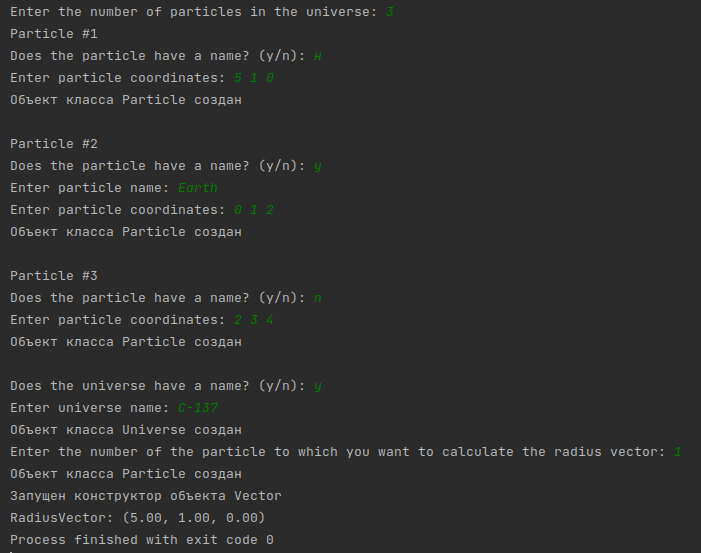
\includegraphics[width=0.8\textwidth]{output.png}
\caption{Результат}
\label{fig:output}
\end{figure}

\end{document}